\frame
{
\frametitle{Respuestas al plan de riesgos}

\begin{block}{Definición}
	Es el proceso de \textbf{desarrollo} de opciones y \textbf{oportunidades} para mejorar
	y reducir las \textbf{amenazas} a los objetivos del proyecto.
\end{block}
}

\frame
{
\frametitle{Respuestas al plan de riesgos}
\framesubtitle{Entradas}
\begin{columns}
	\begin{column}{0.8\textwidth}
		\begin{itemize}
			\item <1-> \textbf{Registro} de Riesgos
			\item <2-> \textbf{Plan} de Administración de Riesgos
		\end{itemize}
	\end{column}
	\begin{column}{0.2\textwidth}
		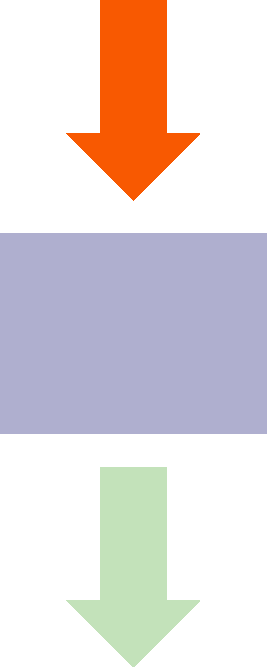
\includegraphics[width=2cm]{img/input}
	\end{column}
\end{columns}
}

%\frame
%{
%\frametitle{Respuestas al plan de riesgos}
%\framesubtitle{Herramientas y Técnicas}
%%Es necesario esto? quizas solo con el itemize basta.
%Varias estrategias de respuesta al riesgo están disponibles.
%La estrategia o combinación de estrategias más probable que sea eficaz
%ha de ser seleccionadas para cada riesgo. herramientas de análisis de
%riesgos, como el análisis de árbol de decisión, puede ser utilizado
%para elegir las respuestas más apropiadas.
%}

\frame
{
\frametitle{Respuestas al plan de riesgos}
\framesubtitle{Herramientas y Técnicas}

\begin{columns}
	\begin{column}{0.8\textwidth}
		\begin{itemize}
			\item <1-> Estrategias para Riesgos Negativos o \textbf{Amenazas}
				\begin{itemize}
					\item <2-> \textbf{Evitar}.
					\item <3-> \textbf{Transferencia}.
					\item <4-> \textbf{Mitigar}.
					\item <5-> \textbf{Aceptar}.
				\end{itemize}
			\item <6-> Estrategias para Riesgos Positivos u \textbf{Oportunidades}
				\begin{itemize}
					\item <7-> \textbf{Explotar}.
					\item <8-> \textbf{Compartir}.
					\item <9-> \textbf{Mejorar}.
					\item <10-> \textbf{Aceptar}.
				\end{itemize}
		\end{itemize}
	\end{column}
	\begin{column}{0.2\textwidth}
		\includegraphics[width=2cm]{img/tools}
	\end{column}
\end{columns}
}

\frame
{
\frametitle{Respuestas al plan de riesgos}
\framesubtitle{Herramientas y Técnicas}
\begin{columns}
	\begin{column}{0.8\textwidth}
		\begin{itemize}
			\item <1-> Estrategias de Respuestas de \textbf{Contingencias}
			\item <2-> Juicio \textbf{Experto}
		\end{itemize}
	\end{column}
	\begin{column}{0.2\textwidth}
		\includegraphics[width=2cm]{img/tools}
	\end{column}
\end{columns}
}

\frame
{
\frametitle{Respuestas al plan de riesgos}
\framesubtitle{Salidas}
\begin{columns}
	\begin{column}{0.8\textwidth}
		\begin{itemize}
			\item <1-> \textbf{Actualizaciones} de Registro de Riesgos
			\item <2-> Decisiones de \textbf{contrato} relacionadas a Riesgos
			\item <3-> \textbf{Actualizaciones} a Plan de Administración de Proyecto
			\item <4-> \textbf{Actualizaciones} al Documento de Proyecto
		\end{itemize}
	\end{column}
	\begin{column}{0.2\textwidth}
		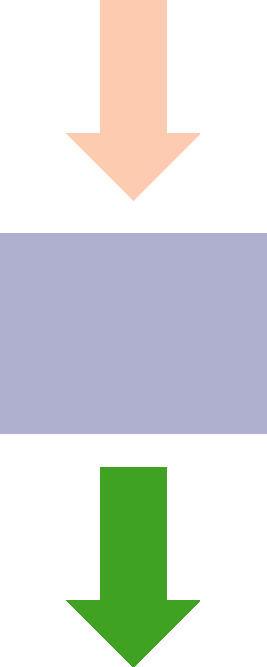
\includegraphics[width=2cm]{img/output}
	\end{column}
\end{columns}
}
